% Options for packages loaded elsewhere
\PassOptionsToPackage{unicode}{hyperref}
\PassOptionsToPackage{hyphens}{url}
\PassOptionsToPackage{dvipsnames,svgnames,x11names}{xcolor}
%
\documentclass[
  letterpaper,
  DIV=11,
  numbers=noendperiod]{scrartcl}

\usepackage{amsmath,amssymb}
\usepackage{lmodern}
\usepackage{iftex}
\ifPDFTeX
  \usepackage[T1]{fontenc}
  \usepackage[utf8]{inputenc}
  \usepackage{textcomp} % provide euro and other symbols
\else % if luatex or xetex
  \usepackage{unicode-math}
  \defaultfontfeatures{Scale=MatchLowercase}
  \defaultfontfeatures[\rmfamily]{Ligatures=TeX,Scale=1}
\fi
% Use upquote if available, for straight quotes in verbatim environments
\IfFileExists{upquote.sty}{\usepackage{upquote}}{}
\IfFileExists{microtype.sty}{% use microtype if available
  \usepackage[]{microtype}
  \UseMicrotypeSet[protrusion]{basicmath} % disable protrusion for tt fonts
}{}
\makeatletter
\@ifundefined{KOMAClassName}{% if non-KOMA class
  \IfFileExists{parskip.sty}{%
    \usepackage{parskip}
  }{% else
    \setlength{\parindent}{0pt}
    \setlength{\parskip}{6pt plus 2pt minus 1pt}}
}{% if KOMA class
  \KOMAoptions{parskip=half}}
\makeatother
\usepackage{xcolor}
\setlength{\emergencystretch}{3em} % prevent overfull lines
\setcounter{secnumdepth}{-\maxdimen} % remove section numbering
% Make \paragraph and \subparagraph free-standing
\ifx\paragraph\undefined\else
  \let\oldparagraph\paragraph
  \renewcommand{\paragraph}[1]{\oldparagraph{#1}\mbox{}}
\fi
\ifx\subparagraph\undefined\else
  \let\oldsubparagraph\subparagraph
  \renewcommand{\subparagraph}[1]{\oldsubparagraph{#1}\mbox{}}
\fi

\usepackage{color}
\usepackage{fancyvrb}
\newcommand{\VerbBar}{|}
\newcommand{\VERB}{\Verb[commandchars=\\\{\}]}
\DefineVerbatimEnvironment{Highlighting}{Verbatim}{commandchars=\\\{\}}
% Add ',fontsize=\small' for more characters per line
\usepackage{framed}
\definecolor{shadecolor}{RGB}{241,243,245}
\newenvironment{Shaded}{\begin{snugshade}}{\end{snugshade}}
\newcommand{\AlertTok}[1]{\textcolor[rgb]{0.68,0.00,0.00}{#1}}
\newcommand{\AnnotationTok}[1]{\textcolor[rgb]{0.37,0.37,0.37}{#1}}
\newcommand{\AttributeTok}[1]{\textcolor[rgb]{0.40,0.45,0.13}{#1}}
\newcommand{\BaseNTok}[1]{\textcolor[rgb]{0.68,0.00,0.00}{#1}}
\newcommand{\BuiltInTok}[1]{\textcolor[rgb]{0.00,0.23,0.31}{#1}}
\newcommand{\CharTok}[1]{\textcolor[rgb]{0.13,0.47,0.30}{#1}}
\newcommand{\CommentTok}[1]{\textcolor[rgb]{0.37,0.37,0.37}{#1}}
\newcommand{\CommentVarTok}[1]{\textcolor[rgb]{0.37,0.37,0.37}{\textit{#1}}}
\newcommand{\ConstantTok}[1]{\textcolor[rgb]{0.56,0.35,0.01}{#1}}
\newcommand{\ControlFlowTok}[1]{\textcolor[rgb]{0.00,0.23,0.31}{#1}}
\newcommand{\DataTypeTok}[1]{\textcolor[rgb]{0.68,0.00,0.00}{#1}}
\newcommand{\DecValTok}[1]{\textcolor[rgb]{0.68,0.00,0.00}{#1}}
\newcommand{\DocumentationTok}[1]{\textcolor[rgb]{0.37,0.37,0.37}{\textit{#1}}}
\newcommand{\ErrorTok}[1]{\textcolor[rgb]{0.68,0.00,0.00}{#1}}
\newcommand{\ExtensionTok}[1]{\textcolor[rgb]{0.00,0.23,0.31}{#1}}
\newcommand{\FloatTok}[1]{\textcolor[rgb]{0.68,0.00,0.00}{#1}}
\newcommand{\FunctionTok}[1]{\textcolor[rgb]{0.28,0.35,0.67}{#1}}
\newcommand{\ImportTok}[1]{\textcolor[rgb]{0.00,0.46,0.62}{#1}}
\newcommand{\InformationTok}[1]{\textcolor[rgb]{0.37,0.37,0.37}{#1}}
\newcommand{\KeywordTok}[1]{\textcolor[rgb]{0.00,0.23,0.31}{#1}}
\newcommand{\NormalTok}[1]{\textcolor[rgb]{0.00,0.23,0.31}{#1}}
\newcommand{\OperatorTok}[1]{\textcolor[rgb]{0.37,0.37,0.37}{#1}}
\newcommand{\OtherTok}[1]{\textcolor[rgb]{0.00,0.23,0.31}{#1}}
\newcommand{\PreprocessorTok}[1]{\textcolor[rgb]{0.68,0.00,0.00}{#1}}
\newcommand{\RegionMarkerTok}[1]{\textcolor[rgb]{0.00,0.23,0.31}{#1}}
\newcommand{\SpecialCharTok}[1]{\textcolor[rgb]{0.37,0.37,0.37}{#1}}
\newcommand{\SpecialStringTok}[1]{\textcolor[rgb]{0.13,0.47,0.30}{#1}}
\newcommand{\StringTok}[1]{\textcolor[rgb]{0.13,0.47,0.30}{#1}}
\newcommand{\VariableTok}[1]{\textcolor[rgb]{0.07,0.07,0.07}{#1}}
\newcommand{\VerbatimStringTok}[1]{\textcolor[rgb]{0.13,0.47,0.30}{#1}}
\newcommand{\WarningTok}[1]{\textcolor[rgb]{0.37,0.37,0.37}{\textit{#1}}}

\providecommand{\tightlist}{%
  \setlength{\itemsep}{0pt}\setlength{\parskip}{0pt}}\usepackage{longtable,booktabs,array}
\usepackage{calc} % for calculating minipage widths
% Correct order of tables after \paragraph or \subparagraph
\usepackage{etoolbox}
\makeatletter
\patchcmd\longtable{\par}{\if@noskipsec\mbox{}\fi\par}{}{}
\makeatother
% Allow footnotes in longtable head/foot
\IfFileExists{footnotehyper.sty}{\usepackage{footnotehyper}}{\usepackage{footnote}}
\makesavenoteenv{longtable}
\usepackage{graphicx}
\makeatletter
\def\maxwidth{\ifdim\Gin@nat@width>\linewidth\linewidth\else\Gin@nat@width\fi}
\def\maxheight{\ifdim\Gin@nat@height>\textheight\textheight\else\Gin@nat@height\fi}
\makeatother
% Scale images if necessary, so that they will not overflow the page
% margins by default, and it is still possible to overwrite the defaults
% using explicit options in \includegraphics[width, height, ...]{}
\setkeys{Gin}{width=\maxwidth,height=\maxheight,keepaspectratio}
% Set default figure placement to htbp
\makeatletter
\def\fps@figure{htbp}
\makeatother

\KOMAoption{captions}{tableheading}
\makeatletter
\makeatother
\makeatletter
\makeatother
\makeatletter
\@ifpackageloaded{caption}{}{\usepackage{caption}}
\AtBeginDocument{%
\ifdefined\contentsname
  \renewcommand*\contentsname{Table of contents}
\else
  \newcommand\contentsname{Table of contents}
\fi
\ifdefined\listfigurename
  \renewcommand*\listfigurename{List of Figures}
\else
  \newcommand\listfigurename{List of Figures}
\fi
\ifdefined\listtablename
  \renewcommand*\listtablename{List of Tables}
\else
  \newcommand\listtablename{List of Tables}
\fi
\ifdefined\figurename
  \renewcommand*\figurename{Figure}
\else
  \newcommand\figurename{Figure}
\fi
\ifdefined\tablename
  \renewcommand*\tablename{Table}
\else
  \newcommand\tablename{Table}
\fi
}
\@ifpackageloaded{float}{}{\usepackage{float}}
\floatstyle{ruled}
\@ifundefined{c@chapter}{\newfloat{codelisting}{h}{lop}}{\newfloat{codelisting}{h}{lop}[chapter]}
\floatname{codelisting}{Listing}
\newcommand*\listoflistings{\listof{codelisting}{List of Listings}}
\makeatother
\makeatletter
\@ifpackageloaded{caption}{}{\usepackage{caption}}
\@ifpackageloaded{subcaption}{}{\usepackage{subcaption}}
\makeatother
\makeatletter
\@ifpackageloaded{tcolorbox}{}{\usepackage[many]{tcolorbox}}
\makeatother
\makeatletter
\@ifundefined{shadecolor}{\definecolor{shadecolor}{rgb}{.97, .97, .97}}
\makeatother
\makeatletter
\makeatother
\ifLuaTeX
  \usepackage{selnolig}  % disable illegal ligatures
\fi
\IfFileExists{bookmark.sty}{\usepackage{bookmark}}{\usepackage{hyperref}}
\IfFileExists{xurl.sty}{\usepackage{xurl}}{} % add URL line breaks if available
\urlstyle{same} % disable monospaced font for URLs
\hypersetup{
  pdftitle={Preliminary Results},
  pdfauthor={Adelle Molina},
  colorlinks=true,
  linkcolor={blue},
  filecolor={Maroon},
  citecolor={Blue},
  urlcolor={Blue},
  pdfcreator={LaTeX via pandoc}}

\title{Preliminary Results}
\author{Adelle Molina}
\date{}

\begin{document}
\maketitle
\ifdefined\Shaded\renewenvironment{Shaded}{\begin{tcolorbox}[borderline west={3pt}{0pt}{shadecolor}, breakable, boxrule=0pt, enhanced, interior hidden, frame hidden, sharp corners]}{\end{tcolorbox}}\fi

\hypertarget{boosted-regression-trees-for-herring-recruitment}{%
\subsection{Boosted Regression Trees for herring
recruitment}\label{boosted-regression-trees-for-herring-recruitment}}

Code for getting data, generating time series of possible variables,
correlation matrices, and boosted regression trees (preliminary results)

\hypertarget{load-packages}{%
\subsubsection{Load packages}\label{load-packages}}

\hypertarget{load-data}{%
\subsubsection{Load data}\label{load-data}}

Data came from various sources (mostly ecodata github) and were
modified, summarized, compiled and exported in a separate script.

\begin{itemize}
\tightlist
\item
  SST \& BT raw data came from the NMFS survey and were clipped to EPU
  regions

  \begin{itemize}
  \tightlist
  \item
    Annual survey derived SST and BT were area weighted
  \end{itemize}
\item
  Annual and/or regional environmental indices came from ecodata

  \begin{enumerate}
  \def\labelenumi{\arabic{enumi}.}
  \item
    heatwave
  \item
    cold pool
  \item
    gulf stream index
  \end{enumerate}
\item
  Various zooplankton indices came ecodata and include abundance,
  density, and copepod abundance
\item
  Recruitment indices came from ASAP model run
\item
  Other indices, such as salinity and chlorophyll would require a
  separate analysis b/c time series are shorter
\end{itemize}

\hypertarget{preliminary-plots}{%
\subsubsection{Preliminary plots}\label{preliminary-plots}}

Plot time series of possible variables and correlation matrices.

\begin{Shaded}
\begin{Highlighting}[]
\CommentTok{\# Temperature}
\NormalTok{temp.dat }\OtherTok{\textless{}{-}}\NormalTok{ dat}\SpecialCharTok{\%\textgreater{}\%} 
\NormalTok{  dplyr}\SpecialCharTok{::}\FunctionTok{select}\NormalTok{(year, }\FunctionTok{c}\NormalTok{(}\FunctionTok{names}\NormalTok{(dat)[}\DecValTok{9}\SpecialCharTok{:}\DecValTok{23}\NormalTok{]),SPR, logR.dev, Rs)}
\NormalTok{temps.melt }\OtherTok{\textless{}{-}}\NormalTok{ reshape2}\SpecialCharTok{::}\FunctionTok{melt}\NormalTok{(temp.dat, }\AttributeTok{id.vars=}\StringTok{"year"}\NormalTok{, }\AttributeTok{variable.name=}\StringTok{"series"}\NormalTok{)}

\FunctionTok{ggplot}\NormalTok{(temps.melt, }\FunctionTok{aes}\NormalTok{(year,value)) }\SpecialCharTok{+}
  \FunctionTok{geom\_line}\NormalTok{()}\SpecialCharTok{+} 
  \FunctionTok{theme\_bw}\NormalTok{()}\SpecialCharTok{+}
  \FunctionTok{facet\_wrap}\NormalTok{(}\SpecialCharTok{\textasciitilde{}}\NormalTok{ series, }\AttributeTok{scales =} \StringTok{"free"}\NormalTok{, }\AttributeTok{ncol=}\DecValTok{4}\NormalTok{)}
\end{Highlighting}
\end{Shaded}

\begin{figure}[H]

{\centering \includegraphics{Preliminary-Results_files/figure-pdf/Plot-data-1.pdf}

}

\end{figure}

\begin{Shaded}
\begin{Highlighting}[]
\NormalTok{ggstatsplot}\SpecialCharTok{::}\FunctionTok{ggcorrmat}\NormalTok{(}
  \AttributeTok{data =}\NormalTok{ temp.dat,}
  \AttributeTok{type =} \StringTok{"nonparametric"}\NormalTok{, }
  \AttributeTok{colors =} \FunctionTok{c}\NormalTok{(}\StringTok{"darkred"}\NormalTok{, }\StringTok{"white"}\NormalTok{, }\StringTok{"steelblue"}\NormalTok{))}
\end{Highlighting}
\end{Shaded}

\begin{figure}[H]

{\centering \includegraphics{Preliminary-Results_files/figure-pdf/Plot-data-2.pdf}

}

\end{figure}

\begin{Shaded}
\begin{Highlighting}[]
\CommentTok{\# Environmental Indices}
\NormalTok{env.dat}\OtherTok{\textless{}{-}}\NormalTok{ dat}\SpecialCharTok{\%\textgreater{}\%} 
\NormalTok{  dplyr}\SpecialCharTok{::}\FunctionTok{select}\NormalTok{(year, }\FunctionTok{c}\NormalTok{(}\FunctionTok{names}\NormalTok{(dat)[}\DecValTok{23}\SpecialCharTok{:}\DecValTok{28}\NormalTok{]),SPR, logR.dev, Rs)}
\NormalTok{env.melt }\OtherTok{\textless{}{-}}\NormalTok{ reshape2}\SpecialCharTok{::}\FunctionTok{melt}\NormalTok{(env.dat, }\AttributeTok{id.vars=}\StringTok{"year"}\NormalTok{, }\AttributeTok{variable.name=}\StringTok{"series"}\NormalTok{)}
\FunctionTok{ggplot}\NormalTok{(env.melt, }\FunctionTok{aes}\NormalTok{(year,value)) }\SpecialCharTok{+}
  \FunctionTok{geom\_line}\NormalTok{()}\SpecialCharTok{+} 
  \FunctionTok{theme\_bw}\NormalTok{()}\SpecialCharTok{+}
  \FunctionTok{facet\_wrap}\NormalTok{(}\SpecialCharTok{\textasciitilde{}}\NormalTok{ series, }\AttributeTok{scales =} \StringTok{"free"}\NormalTok{, }\AttributeTok{ncol=}\DecValTok{4}\NormalTok{)}
\end{Highlighting}
\end{Shaded}

\begin{figure}[H]

{\centering \includegraphics{Preliminary-Results_files/figure-pdf/Plot-data-3.pdf}

}

\end{figure}

\begin{Shaded}
\begin{Highlighting}[]
\NormalTok{ggstatsplot}\SpecialCharTok{::}\FunctionTok{ggcorrmat}\NormalTok{(}
  \AttributeTok{data =}\NormalTok{ env.dat,}
  \AttributeTok{type =} \StringTok{"nonparametric"}\NormalTok{, }
  \AttributeTok{colors =} \FunctionTok{c}\NormalTok{(}\StringTok{"darkred"}\NormalTok{, }\StringTok{"white"}\NormalTok{, }\StringTok{"steelblue"}\NormalTok{))}
\end{Highlighting}
\end{Shaded}

\begin{figure}[H]

{\centering \includegraphics{Preliminary-Results_files/figure-pdf/Plot-data-4.pdf}

}

\end{figure}

\begin{Shaded}
\begin{Highlighting}[]
\DocumentationTok{\#\# \# Biological }
\NormalTok{bio.dat }\OtherTok{\textless{}{-}}\NormalTok{ dat}\SpecialCharTok{\%\textgreater{}\%} 
\NormalTok{  dplyr}\SpecialCharTok{::}\FunctionTok{select}\NormalTok{(year,  }\FunctionTok{c}\NormalTok{(}\FunctionTok{names}\NormalTok{(dat)[}\DecValTok{29}\SpecialCharTok{:}\DecValTok{39}\NormalTok{]),SPR, logR.dev, Rs)}
\NormalTok{bio.melt }\OtherTok{\textless{}{-}}\NormalTok{ reshape2}\SpecialCharTok{::}\FunctionTok{melt}\NormalTok{(bio.dat, }\AttributeTok{id.vars=}\StringTok{"year"}\NormalTok{, }\AttributeTok{variable.name=}\StringTok{"series"}\NormalTok{)}
\FunctionTok{ggplot}\NormalTok{(bio.melt, }\FunctionTok{aes}\NormalTok{(year,value)) }\SpecialCharTok{+}
  \FunctionTok{geom\_line}\NormalTok{()}\SpecialCharTok{+} 
  \FunctionTok{theme\_bw}\NormalTok{()}\SpecialCharTok{+}
  \FunctionTok{facet\_wrap}\NormalTok{(}\SpecialCharTok{\textasciitilde{}}\NormalTok{ series, }\AttributeTok{scales =} \StringTok{"free"}\NormalTok{, }\AttributeTok{ncol=}\DecValTok{4}\NormalTok{)}
\end{Highlighting}
\end{Shaded}

\begin{figure}[H]

{\centering \includegraphics{Preliminary-Results_files/figure-pdf/Plot-data-5.pdf}

}

\end{figure}

\begin{Shaded}
\begin{Highlighting}[]
\NormalTok{ggstatsplot}\SpecialCharTok{::}\FunctionTok{ggcorrmat}\NormalTok{(}
  \AttributeTok{data =}\NormalTok{ bio.dat,}
  \AttributeTok{type =} \StringTok{"nonparametric"}\NormalTok{,}
  \AttributeTok{colors =} \FunctionTok{c}\NormalTok{(}\StringTok{"darkred"}\NormalTok{, }\StringTok{"white"}\NormalTok{, }\StringTok{"steelblue"}\NormalTok{))}
\end{Highlighting}
\end{Shaded}

\begin{figure}[H]

{\centering \includegraphics{Preliminary-Results_files/figure-pdf/Plot-data-6.pdf}

}

\end{figure}

Most significant correlations are between spawner per recruit and GOM
and/or GB temperature (SST, HW, BT). No significant correlations with
biological indices.

\hypertarget{add-lags}{%
\subsubsection{Add lags}\label{add-lags}}

Prepare data for BRTs --\textgreater{} add lags to the variables and
then join back with the herring data

\hypertarget{run-boosted-regression-trees}{%
\subsubsection{Run Boosted Regression
Trees}\label{run-boosted-regression-trees}}

\begin{Shaded}
\begin{Highlighting}[]
\FunctionTok{ncol}\NormalTok{(brtdat) }\CommentTok{\# how many columns}
\end{Highlighting}
\end{Shaded}

\begin{verbatim}
[1] 96
\end{verbatim}

\begin{Shaded}
\begin{Highlighting}[]
\FunctionTok{which}\NormalTok{(}\FunctionTok{colnames}\NormalTok{(brtdat)}\SpecialCharTok{==}\StringTok{"SPR"}\NormalTok{) }\CommentTok{\# which column is SPR, the dependent variable}
\end{Highlighting}
\end{Shaded}

\begin{verbatim}
[1] 7
\end{verbatim}

\begin{Shaded}
\begin{Highlighting}[]
\NormalTok{brd.mod }\OtherTok{\textless{}{-}}\FunctionTok{gbm.step}\NormalTok{(}\AttributeTok{data=}\NormalTok{brtdat,}
              \AttributeTok{gbm.x=}\FunctionTok{c}\NormalTok{(}\DecValTok{9}\SpecialCharTok{:}\DecValTok{96}\NormalTok{), }\CommentTok{\# Select all columns after herring r indices}
              \AttributeTok{gbm.y=}\DecValTok{7}\NormalTok{, }\CommentTok{\# Spawner per recruit}
              \AttributeTok{family=}\StringTok{"gaussian"}\NormalTok{,}
              \AttributeTok{tree.complexity=}\DecValTok{1}\NormalTok{, }\CommentTok{\# (1 = no interactions)}
              \AttributeTok{learning.rate=}\FloatTok{0.01}\NormalTok{,}
              \AttributeTok{bag.fraction=}\FloatTok{0.7}\NormalTok{)}
\end{Highlighting}
\end{Shaded}

\begin{verbatim}

 
 GBM STEP - version 2.9 
 
Performing cross-validation optimisation of a boosted regression tree model 
for SPR and using a family of gaussian 
Using 37 observations and 88 predictors 
creating 10 initial models of 50 trees 

 folds are unstratified 
total mean deviance =  0.0014 
tolerance is fixed at  0 
ntrees resid. dev. 
50    0.0013 
now adding trees... 
100   0.0012 
150   0.0012 
200   0.0011 
250   0.0011 
300   0.0011 
350   0.0011 
400   0.0011 
450   0.0011 
500   0.001 
550   0.001 
600   0.001 
650   0.001 
700   0.001 
750   0.001 
800   0.001 
850   0.001 
900   0.001 
950   0.001 
1000   0.001 
1050   0.001 
1100   0.001 
1150   0.001 
1200   0.001 
1250   0.001 
1300   0.001 
1350   0.001 
1400   0.001 
1450   0.001 
1500   0.001 
1550   0.001 
1600   0.001 
1650   0.001 
1700   0.001 
1750   0.001 
1800   0.001 
1850   0.001 
1900   0.001 
1950   0.001 
2000   0.001 
2050   0.001 
2100   0.001 
2150   0.001 
2200   0.001 
2250   0.001 
2300   0.001 
2350   0.001 
2400   0.001 
2450   0.001 
2500   0.001 
2550   0.001 
2600   0.001 
2650   0.001 
2700   0.001 
\end{verbatim}

\begin{verbatim}
fitting final gbm model with a fixed number of 2200 trees for SPR
\end{verbatim}

\begin{figure}[H]

{\centering 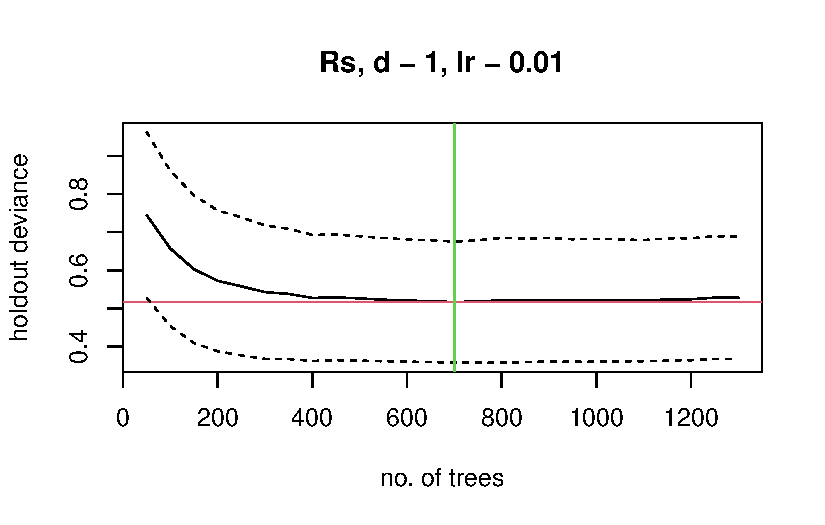
\includegraphics{Preliminary-Results_files/figure-pdf/Boosted Regression Trees-1.pdf}

}

\end{figure}

\begin{verbatim}

mean total deviance = 0.001 
mean residual deviance = 0.001 
 
estimated cv deviance = 0.001 ; se = 0 
 
training data correlation = 0.721 
cv correlation =  0.544 ; se = 0.163 
 
elapsed time -  0.06 minutes 
\end{verbatim}

\begin{Shaded}
\begin{Highlighting}[]
\FunctionTok{summary}\NormalTok{(brd.mod)}
\end{Highlighting}
\end{Shaded}

\begin{verbatim}
                  var      rel.inf
Num.GOM_3   Num.GOM_3 11.686319439
SST.GB_3     SST.GB_3  7.972274623
BT.GOM_3     BT.GOM_3  6.203286931
Num.MAB_3   Num.MAB_3  5.913738518
Surv.BT_3   Surv.BT_3  5.620564043
Num.GB_3     Num.GB_3  5.432611659
Abund_3       Abund_3  4.946851099
OISST_3       OISST_3  4.290000655
SST.SS_3     SST.SS_3  4.264221566
Num.GB_2     Num.GB_2  3.951468599
Surv.SST_3 Surv.SST_3  3.909998540
SST.MAB_3   SST.MAB_3  3.702902856
SST.GOM_3   SST.GOM_3  3.662866951
BT.SS_3       BT.SS_3  3.541432651
BT.MAB_3     BT.MAB_3  3.400286817
BT.GOM_2     BT.GOM_2  2.816115579
BT.GB_3       BT.GB_3  2.742203315
Abund_2       Abund_2  2.681553166
Num.MAB_2   Num.MAB_2  2.463704498
cal.GB_3     cal.GB_3  1.856318509
Num.GOM_2   Num.GOM_2  1.553907278
OISST_2       OISST_2  1.315813400
cal.GOM_3   cal.GOM_3  0.856068106
SST.GOM_2   SST.GOM_2  0.731869902
SST.SS_2     SST.SS_2  0.725382811
BT.SS_2       BT.SS_2  0.565111970
Surv.BT_2   Surv.BT_2  0.530527559
SST.GB_1     SST.GB_1  0.475469336
BT.GB_1       BT.GB_1  0.437477737
cal.GB_2     cal.GB_2  0.301504169
BT.SS_1       BT.SS_1  0.204835110
BT.GB_2       BT.GB_2  0.201331431
cal.GOM_2   cal.GOM_2  0.154122138
BT.GOM_1     BT.GOM_1  0.139724836
Num.MAB_1   Num.MAB_1  0.136169023
SST.SS_1     SST.SS_1  0.088401660
OISST_1       OISST_1  0.071284696
Surv.SST_2 Surv.SST_2  0.057308157
Surv.BT_1   Surv.BT_1  0.051906633
SST.MAB_2   SST.MAB_2  0.051012883
Abund_1       Abund_1  0.045873300
cal.GB_1     cal.GB_1  0.045193339
cal.GOM_1   cal.GOM_1  0.044516862
HW_1             HW_1  0.044216291
BT.MAB_2     BT.MAB_2  0.025899879
Surv.SST_1 Surv.SST_1  0.022428271
Num.GOM_1   Num.GOM_1  0.022320509
HW.MAB_3     HW.MAB_3  0.008433163
HW                 HW  0.007008582
Surv.BT       Surv.BT  0.005809694
Abund           Abund  0.005402260
Num.GB         Num.GB  0.005140504
cal.GB         cal.GB  0.004350723
BT.SS           BT.SS  0.004306856
BT.MAB         BT.MAB  0.001150919
OISST           OISST  0.000000000
Surv.SST     Surv.SST  0.000000000
BT.GB           BT.GB  0.000000000
BT.GOM         BT.GOM  0.000000000
SST.GB         SST.GB  0.000000000
SST.GOM       SST.GOM  0.000000000
SST.MAB       SST.MAB  0.000000000
SST.SS         SST.SS  0.000000000
HW.GB           HW.GB  0.000000000
HW.GOM         HW.GOM  0.000000000
HW.MAB         HW.MAB  0.000000000
Num.GOM       Num.GOM  0.000000000
Num.MAB       Num.MAB  0.000000000
cal.GOM       cal.GOM  0.000000000
cal.SS         cal.SS  0.000000000
BT.MAB_1     BT.MAB_1  0.000000000
SST.GOM_1   SST.GOM_1  0.000000000
SST.MAB_1   SST.MAB_1  0.000000000
HW.GB_1       HW.GB_1  0.000000000
HW.GOM_1     HW.GOM_1  0.000000000
HW.MAB_1     HW.MAB_1  0.000000000
Num.GB_1     Num.GB_1  0.000000000
cal.SS_1     cal.SS_1  0.000000000
SST.GB_2     SST.GB_2  0.000000000
HW_2             HW_2  0.000000000
HW.GB_2       HW.GB_2  0.000000000
HW.GOM_2     HW.GOM_2  0.000000000
HW.MAB_2     HW.MAB_2  0.000000000
cal.SS_2     cal.SS_2  0.000000000
HW_3             HW_3  0.000000000
HW.GB_3       HW.GB_3  0.000000000
HW.GOM_3     HW.GOM_3  0.000000000
cal.SS_3     cal.SS_3  0.000000000
\end{verbatim}

\begin{Shaded}
\begin{Highlighting}[]
\NormalTok{null.dev}\OtherTok{\textless{}{-}}\NormalTok{brd.mod}\SpecialCharTok{$}\NormalTok{self.statistics}\SpecialCharTok{$}\NormalTok{mean.null}
\NormalTok{resid.dev}\OtherTok{\textless{}{-}}\NormalTok{brd.mod}\SpecialCharTok{$}\NormalTok{cv.statistics}\SpecialCharTok{$}\NormalTok{deviance.mean}
\NormalTok{dev.expl}\OtherTok{\textless{}{-}}\NormalTok{((null.dev}\SpecialCharTok{{-}}\NormalTok{resid.dev)}\SpecialCharTok{/}\NormalTok{null.dev)}\SpecialCharTok{*}\DecValTok{100}
\NormalTok{dev.expl}
\end{Highlighting}
\end{Shaded}

\begin{verbatim}
[1] 28.13085
\end{verbatim}

\begin{Shaded}
\begin{Highlighting}[]
\FunctionTok{ggplot}\NormalTok{(}\AttributeTok{data=}\FunctionTok{summary}\NormalTok{(brd.mod),}\FunctionTok{aes}\NormalTok{(}\AttributeTok{x=}\FunctionTok{reorder}\NormalTok{(var,rel.inf),}\AttributeTok{y=}\NormalTok{rel.inf))}\SpecialCharTok{+}
  \FunctionTok{geom\_bar}\NormalTok{(}\AttributeTok{stat=}\StringTok{"identity"}\NormalTok{)}\SpecialCharTok{+}
  \FunctionTok{labs}\NormalTok{(}\AttributeTok{x=}\StringTok{""}\NormalTok{,}\AttributeTok{y=}\StringTok{"relative influence"}\NormalTok{)}\SpecialCharTok{+}
  \FunctionTok{coord\_flip}\NormalTok{()}
\end{Highlighting}
\end{Shaded}

\begin{figure}[H]

{\centering 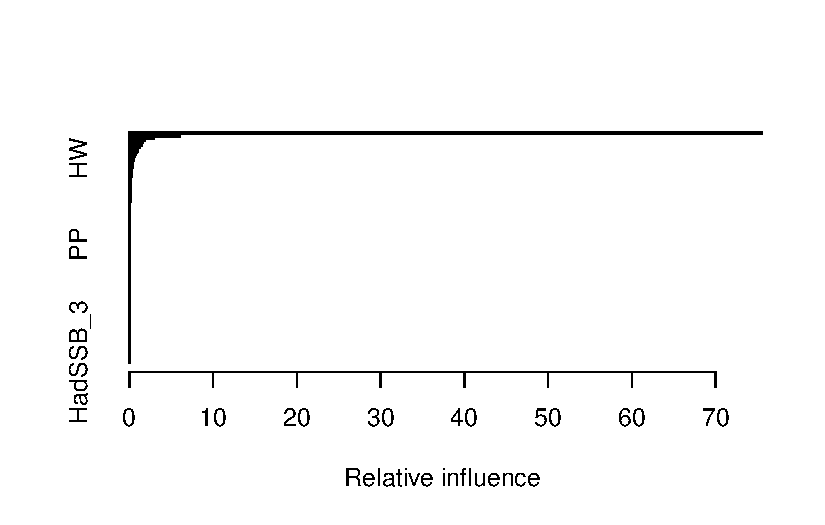
\includegraphics{Preliminary-Results_files/figure-pdf/Boosted Regression Trees-2.pdf}

}

\end{figure}

\begin{figure}[H]

{\centering 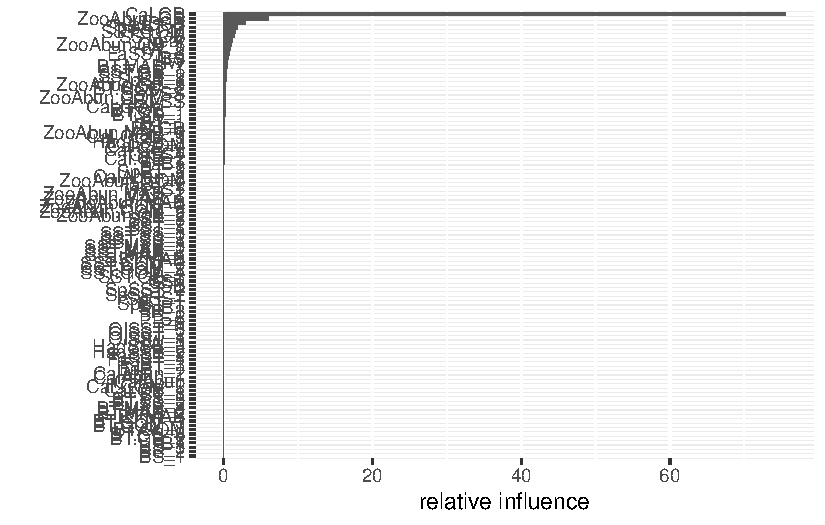
\includegraphics{Preliminary-Results_files/figure-pdf/Boosted Regression Trees-3.pdf}

}

\end{figure}

\begin{itemize}
\item
  Not shown here are different runs with just up to 2 year lags, and
  with no lags

  \begin{itemize}
  \tightlist
  \item
    top variables always include food and temp
  \end{itemize}
\item
  Almost all the top 10 variables include a two year lag and include
  sst, bt, and abundance of copepods in all or either GB and/or GoM
\item
  Ran with more data and found that relative influence of top variables
  changed and instead most top variables have a 3 years lag, but also
  include sst and copepods
\item
  Several variables were not important at all
\end{itemize}



\end{document}
